\chapter{Theoretical Background}
\label{chapter:background}
\begin{music}
    \parindent10mm \instrumentnumber{1} \setstaffs1{1} 
    \generalmeter{\meterfrac34} \generalsignature{-1}
    \startextract
		\notes  \en
    \zendextract
\end{music}
\epigraph{\textit{the passion of friendship will soon blossom into a righteous power}}{Bolero of Fire --- Ocarina of Time}

% Convolutional neural networks trained on large databases \cite{mnist2012,imagenet2009} have shaped machine learning research over the past couple of decades. Today they serve as canonical learning material in courses and are often used as initial \textit{vanilla} approaches for data exploration and classification tasks and before creating more bespoke machine learning pipelines. The widespread success of much models created an expectation in the research community that with sufficient data and computational power provided by one of the reigning consumer internet businesses, a data-driven black-box model can be created for any application ranging from quantum mechanics to economics. Convolutional architectures together with language models eventually inspired recurrent architectures and attention models where are the key ingredients in the creation of \textit{Alpha Fold} \cite{Jumper2021HighlyAlphaFold} that takes a substantial step towards solving the protein-folding problem. Biotechnology researchers are eager to apply these methods but face the following obstacles

% \begin{itemize}
%     \item \textbf{Insufficient data} due to strategic experimental designs 
%     \item \textbf{Low extrapolation accuracy} for black box-models
% \end{itemize}

This Chapter lays out a background bifurcation theory and machine learning methods relevant to cell biology and flow cytometry. We establish the connection between the concept of phenotypes and bifurcations in Section \ref{section:phenotypes-with-bifurcations} and lay out assumptions and definitions that are used throughout other chapters. Section \ref{section:applications-cell-biology} follows up with concrete applications of differential equations in cell biology and will prepare the reader for the incorporated synthetic biology publication in Chapter \ref{chapter:double-exclusive}.

The problem of inferring phenotypes from data is defined in Section \ref{section:phenotype-inference} with a survey relevant machine learning methods. This section discusses the pre-processing techniques to extract bifurcations from raw data, as has been done in Chapter \ref{chapter:double-exclusive}, and used as a starting point in the incorporated machine learning publication in Chapter \ref{chapter:inference}. Section \ref{section:applications-flow-cytometry} gives the reader a background in flow cytometry and how the machine learning methods discussed in previous sections are used by immunologists to identify immune cell phenotypes. This section lays the foundations for the interactive exploration tool presented in Chapter \ref{chapter:exploring}.

\section{Describing Phenotypes with Bifurcations}
\label{section:phenotypes-with-bifurcations}

%Bringing in the definition here is too early. Too abrupt.
A phenotype is a qualitative state or behaviour of an organism that can be described by several quantitative features.
%Historical context of how the word emerged and how it is used in biological contexts

Before considering the additional complexity that comes with biology, let us first consider a simple everyday metaphor: light bulbs. Light bulbs come in various combinations of quantitative features $\theta$ which could be its shape, colour, materials and circuit design. The purpose of a light bulb is to fulfil a single function: increase in brightness as a function of voltage $p$, pushing the qualitative state of the bulb from \emph{off} to \emph{on}. Changes to bulb shape affect neither its function nor its states. Changes in color affect the quality of the \emph{on} state but not the \emph{off} state. Changes to circuit design and materials may change or even break the bulb's function. Fluorescent bulbs, for example, only have two possible brightness states in response to changes in voltage $p$, while incandescent bulbs have a continuous brightness response.
\\
\begin{Figure}
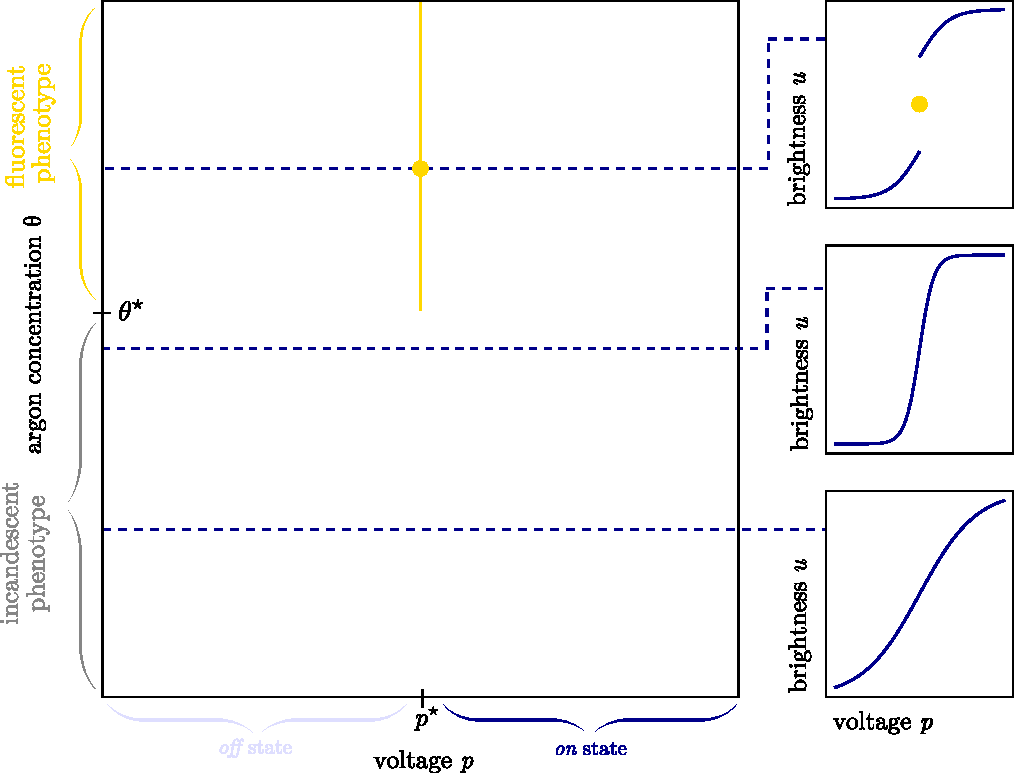
\includegraphics[scale=0.7]{bulb}
\caption{a) The bifurcations (shown in gold) at critical voltage $p^\star$ above argon concentration $\theta^\star$ give rise to sudden jumps in brightness (right-hand panels). $\theta^\star$ separates two bulb phenotypes and $p^\star$ separates the \emph{on} and \emph{off} states.}
\label{fig:bulb}
\end{Figure}

The fluorescent and incandescent bulbs can be considered as two different phenotypes distinguished by the quality of their response to voltage changes. Different colour bulbs can also be considered phenotypes, distinguished by the quality of their \emph{on} state, rather than their response to voltage. Bifurcation theory allows us to describe the transitions between qualitative states and can be leveraged to distinguish and organise phenotypes. In this context a bifurcation becomes a punctuation that either \emph{distinguishes between phenotypes} or \emph{distinguishes between behaviours within a phenotype}.

Suppose we inserted a component into our light bulb that changed parameter $\theta$ in such a way so that we can change between the discrete response of the fluorescent bulb and the continuous response of the incandescent bulb. Perhaps $\theta$ could be the concentration of argon gas; the bulb would have to be wired to behave like an incandescent bulb at low concentrations. We could collect brightness $u$ as a function of voltage $p$ and gas concentration $\theta$ produce something similar to that shown in Figure \ref{fig:bulb}. The bifurcations at critical voltage $p^\star$ above argon concentration $\theta^\star$ give rise to sudden jumps in brightness. The bifurcations separate the \emph{on} and \emph{off} states of the bulb and are only present in the fluorescent phenotype. The two phenotypes lie either side of  the onset of bifurcations at concentration $\theta^\star$. We can see from Figure \ref{fig:bulb} how knowing the locations of bifurcations allows us to organise qualitative behaviours and hence phenotypes of the bulb.

In the biological context, we can consider changes in $\theta$ as changes in the organism genotype that may or may not lead to a new phenotype. The idea of describing phenotypes in this way has been done before by Waddington \cite{}. His epigenetic landscape is a metaphor for how changes gene regulation, in our case represented by changes in $\theta$, determines the fate of cells. He imagines the cell as a marble, rolling down a series of forking valleys representing a differentiation cascade, eventually settling in its final phenotype. Let us adopt this metaphor for organism behaviours in response to a controlled condition (Figure \ref{fig:waddington}). Changing the control condition places the marble at different points in the valley and each fork in the valley corresponds to different available behaviours to the organism. Changing the parameters $\theta$ changes the topology of the valleys potentially giving rise to new behaviours and therefore new phenotypes. Due to the robustness \cite{} and fragility \cite{} of organisms we expect most changes in $\theta$ to either kill the organism or do nothing at all. The emerging picture suggests that the route between phenotypes is a carefully created sequence of changes in $\theta$.

\begin{Figure}
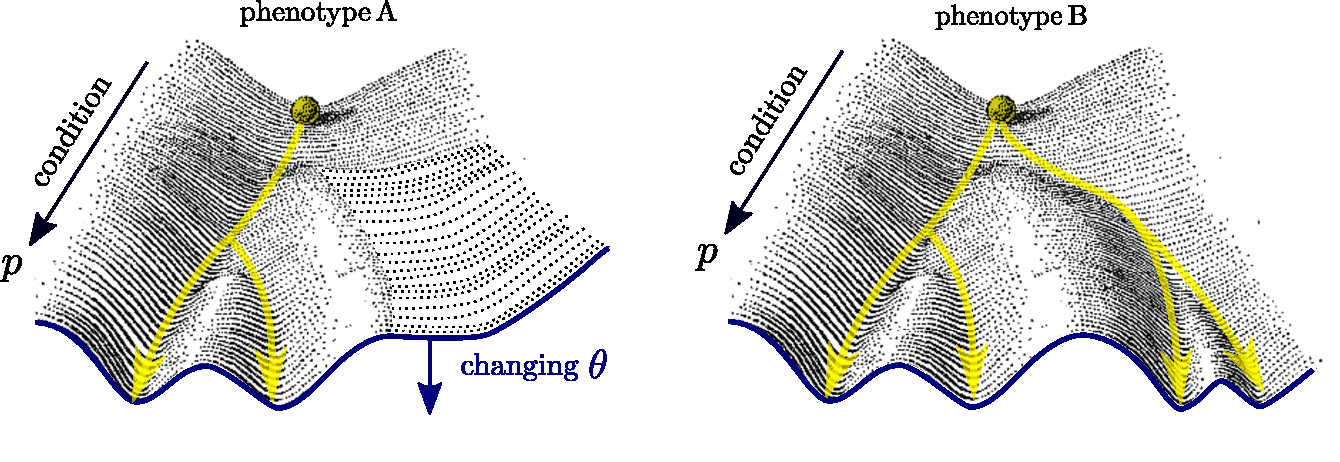
\includegraphics[scale=0.6]{waddington}
\caption{Waddington landscapes representing the set of available behaviours for two phenotypes in response to a controlled condition $p$. Phenotypes are related by changes in landscape topology via changes in $\theta$}
\label{fig:waddington}
\end{Figure}

In order to enumerate the phenotype distribution in the the high-dimensional parameter space $\theta$ for a given organism we must construct a model. By parametrising such a model $\rates(u,p)$ by $\theta$, we can relate the states of the organism $u$ to experimentally controlled conditions $p$. Ideally a subset of $u$ can be observed experimentally so that we may observe bifurcations in the data, as demonstrated in the right-hand panel of Figure \ref{fig:bulb}. In the following section we shall go through a class of models that can leverage bifurcation theory.  

% The problem is that the space of decisions that change $\theta$ is intractably large. Furthermore there is no guarantee that any two phenotypes would be connected via experimentally accessible changes in $\theta$. We will see in the incorporated publication in Chapter \ref{chapter:double-exclusive} how differential equation modelling and machine learning can be used to guide experiments and the genetic engineering of \emph{E. coli} towards a phenotype referred to as the \emph{double exclusive reporter}. 

% In the collaboration, bifurcation theory \cite{} was used to detect the onset of the desired phenotypic behaviour in a set of differential equations that model the engineered genetic circuits in \emph{E. coli}. We will see in the following sections how bifurcation theory is perfectly suited for modelling transitions between phenotypes, and hence popularised in fields such as synthetic biology and ecology. Through the use of machine learning and bifurcation theory in the same collaboration, we identified a gap: \emph{there existed no differentiable machine learning method that leveraged bifurcation theory directly}. The incorporated publication in Chapter \ref{chapter:inference} fills this gap, enabling an efficient exploration of phenotypes in the high-dimensional space of $\theta$.

% The antimicrobial resistance originates from selective pressures in the environment which change biochemical pathways which we can encode in parameters $\theta$. Neurons also have pathways that regulate aspects such as thickness of myelin sheaths on axons, that in turn dictate how sensitive, if at all, they are to firing. In the case of the \emph{Zebrafish} the parameters $\theta$ encode whether a particular mutation in the genome is present or not. 

% Synthetic biologists like to import such engineering metaphors when designing genetic sequences that would produce a desired behaviour. Genetic components are designed to be modular and mass produced like electrical components. with various behaviours are mass produced.

% This could be, for example, a phenotype of antimicrobial resistant bacteria \cite{Baym2016SpatiotemporalLandscapes}. We can break down this observation as follows: a cell can be in the qualitative state of \emph{resistant} or \emph{not resistant} at a certain concentration $p$ of antibiotic. Another example could be that of action potentials in neurons \cite{}. A neuron can either be \emph{firing} or \emph{not firing} in response to a given electro-chemical potential $p$. Whole organism phenotypes, such as pigment patterns \emph{Zebrafish} \cite{}, can also be described this way. In this case the phenotype emerges as the organism develops and therefore we look for emergence of \emph{patterns} or \emph{no patterns} over time $p=t$.

% In practice we can only observe a subset of the states, for example by incorporating fluorescent proteins downstream of the coding sequences of the proteins that participate in the antimicrobial resistance. Incorporating any fluorescent proteins into the host genome contributes to cell burdon and at worst can disrupt the mechanism under study. Therefore incorporation sites much be chosen sparsely such that the qualitative behaviour is still observable in the data.

\clearpage
\subsection{Differential Equation Models}

For the purposes of this thesis we will assume that the behaviour of the organism under study can be cast in terms of differential equations in a $N$ states $u$, $M$ parameters $\theta$ and $P$ control conditions $p$. For now we shall state the general class of models and follow up with concrete biological examples as we explore different types of bifurcations. Throughout the thesis we will consider models of the form

\begin{equation}
	\frac{du}{dt} = \rates(u,p)
	\quad\mathrm{where}\quad
	\begin{cases}
		\quad F: \Reals^{N+P}\rightarrow\Reals^N \\
		\quad \theta\in\Reals^M, u\in\Reals^N, p\in\Reals^P
	\end{cases}
	\label{eq:differential-equations}
\end{equation}

\noindent The total derivative $\frac{du}{dt}$ gives us the rate of change of the states with respect to time $t$ and all variables have been vectorised with the appropriate dimension. In principle the right-hand-side $\rates$ can be arbitrarily complicated, containing spatial derivatives or even machine learning models such as neural networks. We shall see later when such models become relevant in biomedical modelling.

\subsubsection{Trajectories \& Field Geometry}

In principle once equations \eqref{eq:differential-equations} have been written down they can be integrated to obtain trajectories $u(t)$ for various initial conditions $u(t')$. We can write the solution down formally as
\begin{equation}
	u(t) = u(t') + \int_{t'}^{t} \rates(u(s),p)\,\mathrm{d}s
	\label{eq:trajectory}
\end{equation}
Here the integral reveals that in order to determine where the state is at time $t$ we need to sum all the contributions of the function $\rates$ from the initial time $t'$ all the way up to final time $t$. The function $\rates$ depends on the state $u$ and must be updated with the integration variable $s$. This calculation can be interpreted, as shown in Figure \ref{fig:fields}, as choosing an initial point $u'=u(t')$ in a vector field $\rates$ and following the field lines until time $t$ at which the final point $u=u(t)$ has been reached.

\begin{Figure}
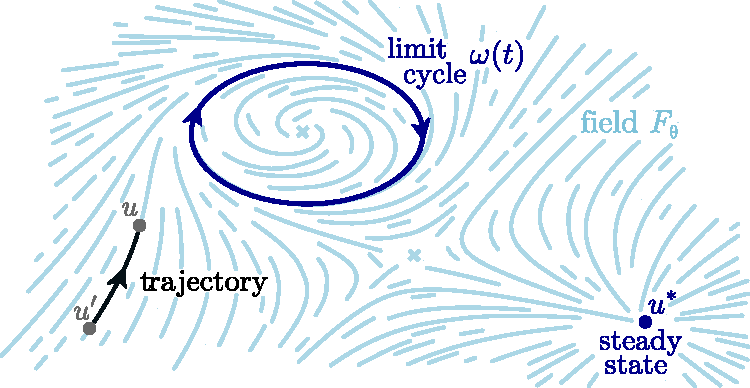
\includegraphics[scale=0.9]{fields}
\caption{Illustration of a trajectory between $u=u(t)$ and $u'=u(t')$ over finite time $t-t'$ following the field lines of $\rates$. In this example field lines either point towards steady state $\steady$ or a limit cycle $\cycle(t)$. There are two unstable fixed points marked by crosses: a saddle point separating the basins of attraction and an unstable focus enclosed by the limit cycle.}
\label{fig:fields}
\end{Figure}

By considering the geometry of the field $\rates$ in state space we can determine the fate of sets of trajectories, which are ultimately pulled towards \emph{dynamical attractors}. Such attractors can be static steady states $\steady$ or dynamic like the limit cycle $\cycle(t)$ illustrated in Figure \ref{fig:fields}. \emph{Dynamical attractors} create basins of attraction defined as regions of state space in which trajectories are pulled towards the same stable structure. These basins must be separated by unstable structures, such as the saddle point marked by a cross in Figure \ref{fig:fields}, which define a boundary between the basins called the separatrix. Note that the direction of the field $\rates$ and not its magnitude $|\rates|$ determines the fate of a trajectories.

When equations \eqref{eq:differential-equations} describe the behaviours of an organism, the attractors determine the set of qualitative behaviours available to the organism of genotype $\theta$, whilst experiencing experimental conditions $p$. If changes to the genotype $\theta$ change the number, type or stability of the attractors then we will observe new qualitative behaviours and hence a new phenotype. If changes to conditions $p$ lead to changes in the state space geometry, this is interpreted as a different behavioural state available to the same phenotype. We can see therefore how casting a biomedical problem into the language of differential equations, allows us to characterise phenotypic traits with the geometry of attractors in state space. 

\subsubsection{The Jacobian Matrix}

In order to quantify the geometry of a local patch of state space $u$ we can imagine $\rates$ as a velocity field of water and place a tiny blob of ink surrounding the location $u$. The so called Jacobian matrix $\jacobian$ of partial derivatives at the location $u$ transforms the basis vectors $\hat u(t)$ defining the blob over a short period of time $\Delta t$ as depicted in Figure \ref{fig:jacobian}. The transformation is
\begin{equation}
	\hat{u}(t+\Delta t)=\left (\mathbb{1}+\jacobian\Delta t \right)\hat{u}(t)
	\quad\mathrm{where}\quad
	\hat{u}\in\Reals^N\quad
	\jacobian\in\Reals^{N\times N}
	\label{eq:jacobian-transformation}
\end{equation}

\begin{Figure}
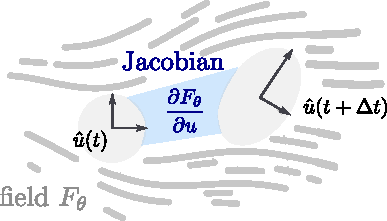
\includegraphics[scale=1.2]{jacobian}
\caption{Illustration how the Jacobian matrix $\jacobian$ transforms the basis vectors $\hat u(t)$ defining a small patch of initial conditions for a short period of time $\Delta t$. The eigenvalues $\lambda$ and eigenvectors $\eigenvector$ define the deformation of the patch}
\label{fig:jacobian}
\end{Figure}
\noindent where $\mathbb{1}$ is the identity matrix. The eigenvalues $\lambda$ and eigenvectors $\eigenvector$ of the Jacobian reveal to us the magnitudes and directions of the stretching or squeezing of the blob. We can diagonalise the Jacobian to obtain the eigenvalues and eigenvectors at any state space location $u$ to quantify the local geometry of the field. The eigenvalue equation is written as

\begin{equation}
	\lambda \eigenvector = \jacobian\eigenvector
	\quad\mathrm{where}\quad
	\eigenvector\in\Reals^N : |\eigenvector|=1
	\label{eq:jacobian-eigenproblem}
\end{equation}
where the eigenvectors are normalised to have unit magnitude. We can take the limit $\Delta t\rightarrow 0$ of equation \eqref{eq:jacobian-transformation} to obtain a first order matrix differential equation for the evolution of basis vectors $\hat u(t)$ in any patch $u$
\begin{equation}
	\frac{d\hat{u}}{dt}=\jacobian\hat{u}
	\label{eq:jacobian-odes}
\end{equation}
The coefficients given by the Jacobian matrix are time-independent and therefore the general solution can be written as a matrix exponential
\begin{equation}
	\hat{u}(t)=\e^{\jacobian(t-t')}\hat{u}(t')
	\label{eq:basis-vector-evolution}
\end{equation}
where $\hat{u}(t')$ are the basis vectors that define the initial shape of the blob centred on location $u$. If we let the basis for the initial blob have axes parallel to the eigenvectors $\eigenvector$ of the Jacobian, then the evolution any vector $\sigma(t)$ within the blob expressed in its basis becomes
\begin{equation}
	\sigma(t)= \sum_{\lambda}\eigenvector
	\sigma_{\lambda}(t') \e^{\lambda(t-t')}
	\label{eq:eigenbasis-vector-evolution}
\end{equation}
where $\sigma_{\lambda}(t')$ are the initial components of the vector in the basis of the blob. This equation reveals explicitly how the sign of real parts to eigenvalues $\Re\mathrm{e}\lambda$ determine the exponential growth or shrinkage of the blob in the direction $\eigenvector$. The imaginary parts $\Im\mathrm{m}\lambda$ determine the magnitude of rotations of the blob. Note that since the Jacobian matrix is real and eigenvalues and eigenvectors appear in conjugate pairs and therefore the overall evolution \eqref{eq:eigenbasis-vector-evolution} yields real transformations of blob vectors $\sigma(t)$.

A field $\rates$ is called \emph{degenerate} in regions of state space $u$ where adjacent field lines do not change and hence do not cause shape changes to the blob in one or more directions. This means that one or more of the eigenvalues of the Jacobian vanish and have associated eigenvectors $\hat\tangent$ that obey
\begin{equation}
	\jacobian \hat\tangent(u) = 0
	\label{eq:tangent-equation}
\end{equation}
This equation constructs vectors $\hat\tangent(u)$ that span the degenerate subspace at field location $u$. Note that a degenerate subspace may not always exist. In linear algebra We will see that this equation is useful not  for constructing tangent spaces,

Equations \eqref{eq:fixed-point-perturbations} suggest that small perturbations away from stable steady states $\steady$ decay exponentially with respect to time. However if the state space flow $\rates$ at the steady state $\steady$ is degenerate, then at least one of the eigenvalues of the Jacobian $\lambda$ vanish. Expanding the exponentials for a subset of $\lambda$ that are close to zero yields

% Suppose we have a vanishing eigenvalue $\lambda(s)$ that we parametrise with $s\in\Reals$ such that $\lambda(s^\star)=0$. This will allow us to explore the dynamics in the vicinity of the degenerate point.

\begin{equation}
	\delta\steady(t)  \approx \sum_{\lambda\approx 0}
	\alpha_{\lambda}\eigenvector(1+\lambda(t-t')+\mathcal{O}(\lambda^2))
	+\sum_{\lambda'\ne\lambda}
	\alpha_{\lambda'}v_{\lambda'}\e^{\lambda'(t-t')}
\end{equation}

This gives rise to relaxation dynamics that are polynomial in the vicinity of the degenerate point along the degenerate directions defined by eigenvectors $\eigenvector$. Perturbations along $v_{\lambda'}$ still decay exponentially and will vanish before the polynomial terms. By considering changes in the magnitude of perturbations $|\delta\steady(t)|-|\delta\steady(t')|$ and dropping higher order terms $\mathcal{O}(\lambda^2)$, and substituting an expression for the eigenvalues we arrive at

\begin{equation}
	\frac{|\delta\steady(t)|-|\delta\steady(t')|}{t-t'}\sim \sum_{\lambda\approx 0}\eigenvector\cdot\left.\jacobian\right|_{\rates(u,p)=0}\!\!\!\!\! \cdot \eigenvector
	\quad\mathrm{where}\quad
	\jacobian \cdot \hat{T}_\theta = 0
\end{equation}

\subsubsection{Lyapunov Spectrum Analysis}

We can determine the stability of attractors by looking at the geometry of field lines in its vicinity. Do they converge or diverge? Does the field rotate? We could answer these questions tracking the evolution of small perturbations $\delta u$ between adjacent trajectories. Let us begin by substituting the perturbed trajectory $u+\delta u$ into equations \eqref{eq:differential-equations}
\begin{equation}
	\frac{d}{dt}(u+\delta u) = \rates(u+\delta u,p)
\end{equation}
After Taylor expanding the field $\rates$ and recognising that equations \eqref{eq:differential-equations} lead to a cancellation in the terms involving the unperturbed trajectory $u$ we arrive at
\begin{equation}
	\frac{d}{dt}(\delta u) =
	\left.\jacobian\right|_{u=u(t)}\!\!\delta u + \mathcal{O}(\delta u^2)
	\label{eq:linearised-differential-equations}
\end{equation}
where $\jacobian$ is the Jacobian of the field and additional terms $\mathcal{O}(\delta u^2)$ involve taking higher order derivatives of the field $\rates$. Choosing a perturbation sufficiently small such that we can ignore higher order terms yields a first order homogenous ordinary matrix differential equation of the form $\dot{\delta u}(t)\approx J(t)\delta u(t)$ where $J(t)$ is a time-varying Jacobian. These equations can be solved formally with time-ordered matrix exponentiation \cite{} 

\begin{Figure}
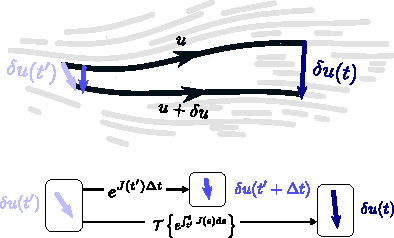
\includegraphics[scale=1.5]{lyapunov}
\caption{Illustration how the time ordering operator $\mathcal{T}\left\{\e^{\int_{t'}^t J(s) \mathrm{d}s}\right\}$ propagates the separation $\delta u(t)$ between adjacent trajectories $u$ and $u+\delta u$ by repeated application of the exponentiated Jacobian $\e^{J(t)\Delta t}$ evaluated along unperturbed trajectory $u(t)$}
\label{fig:lyapunov}
\end{Figure}
\begin{equation}
	\delta u(t) \approx
	\mathcal{T}\left\{\e^{\int_{t'}^t J(s) \mathrm{d}s}\right\}\delta u(t')
	\quad\mathrm{where}\quad
	J(t) := \left.\jacobian\right|_{u=u(t)}
	\label{eq:matrix-exponential}
\end{equation}
The time-ordering defines an ordered product of matrix exponentials
\begin{equation}
	\mathcal{T}\left\{ \e^{\int_{t'}^t J(s) \mathrm{d}s} \right \}:=
	\lim_{\Delta t\rightarrow 0}\left(
		\e^{J(t)\Delta t}\e^{J(t-\Delta t)\Delta t}\,\dots\,
		\e^{J(t'+\Delta t)\Delta t}\e^{J(t')\Delta t}
	\right)
	\label{eq:time-ordering-operator}
\end{equation}
which can be calculated by repeated exponentiation of the Jacobian $\e^{J(t)\Delta t}$ evaluated at different times along the unperturbed trajectory $u(t)$. Although this expression may look complicated it is just another matrix whos eigenvalues reveal whether the trajectories diverge $|\delta u(t\rightarrow\infty)|\rightarrow\infty$ or converge $|\delta u(t\rightarrow\infty)|\rightarrow0$. The rates of convergence or divergence are known as Lyapunov exponents, and can be defined in a local patch of state space $t$ and finite time $\Delta t$ as the eigenvalues of
\begin{equation}
	\Lambda(u,\Delta t) := \frac{1}{\Delta t}\log\left(
		\mathcal{T}\left\{ \e^{\int_{t}^{t+\Delta t} J(s) \mathrm{d}s} \right \}
	\right)
	\label{eq:lyapunov-spectrum}
\end{equation}
Note that to calculate this matrix we need to choose an initial point in state space $u=u(t)$, obtain the trajectory up to $u(t+\Delta t)$ and evaluate the Jacobian along the trajectory in the time ordered integral.

\subsubsection{Linear Stability Analysis}

Thusfar we dealt with stability in arbitrary patches of state space $u$ and asked questions about local flows. What happens when we look at flows in the vicinity of fixed points $\steady$ that satisfy the equation
\begin{equation}
	\left.\frac{du}{dt}\right|_{u=\steady}=\rates(\steady,p) = 0
	\label{eq:fixed-point-equation}
\end{equation}
In this case, since there is no time-dependence in the equation \eqref{eq:matrix-exponential}, the time-ordered integral simplifies yielding a matrix exponential equation for perturbations from fixed points $\delta\steady(t)$
\begin{equation}
	\delta\steady(t) \approx
	\e^{(t-t')\left.\jacobian\right|_{u=\steady}}\delta\steady(t')
	\label{eq:fixed-point-perturbations}
\end{equation}
The Jacobian evaluated at fixed points $\left.\jacobian\right|_{u=\steady}$ can be expressed in terms of its eigenvectors $\eigenvector$ and eigenvalues $\lambda$ and therefore 
\begin{equation}
	\delta\steady(t)  \approx \sum_{\lambda}
	\alpha_{\lambda}\eigenvector \e^{\lambda(t-t')}\quad\mathrm{where}\quad
	\lambda \eigenvector = \eigenvector\cdot\left.\jacobian\right|_{u=\steady} \eigenvector\in\mathbb{S}^{N-1}
\end{equation}
\begin{equation*}
	\mathrm{with}\,\alpha_{\lambda}\,
	\mathrm{given\,\,by\,\,initial\,\,condition}
	\,\delta\steady(t')
	\label{eq:fixed-point-perturbations-diagonal}
\end{equation*}
We can see that the sign of the real parts to eigenvalues $\Re\mathrm{e}\lambda$ determine the exponential growth or shrinkage of fixed point perturbations $\delta\steady(t)$ in the direction parallel to the corresponding eigenvector $\eigenvector$. The imaginary parts $\Im\mathrm{m}\lambda$ determine the frequency of oscillations around the fixed point. If at least one of the eigenvalues has a positive real part $\Re\mathrm{e}\lambda$ the field pushes trajectories away from the fixed point in direction $\eigenvector$ which means the fixed point is unstable.

\begin{Figure}
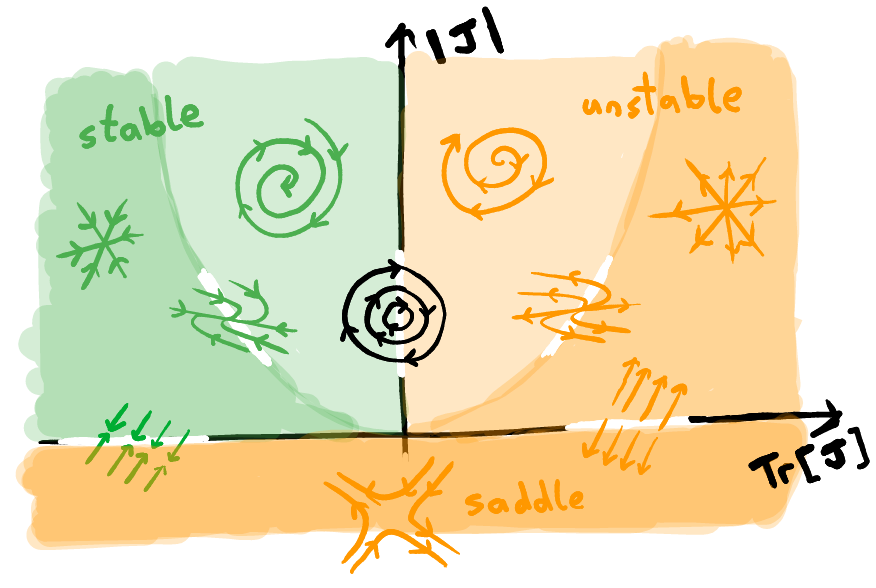
\includegraphics[scale=0.35]{figures/stability}
\caption{Classification of \textcolor{Green}{stable} and \textcolor{orange}{unstable}
fixed points for a general \\two dimensional Jacobian in terms of trace $\mathrm{Tr}[J]$ and
determinant $|J|$}
\label{fig:stability}
\end{Figure}

For a two dimensional system we can express the two eigenvalues of the $2\times 2$ Jacobian in terms of its trace $\mathrm{Tr}[J]$ and determinant $|J|$. Figure \ref{fig:stability} reveals the regions of stability and field flows for an arbitrary two dimensional system in terms of the Jacobian trace and determinant. We can see now how changing the model can lead to changes in sign in one of the eigenvalues of the Jacobian. This leads to a change in stability of a fixed point which is in fact type of bifurcation. This diagram gives us an intuition for the types of fixed points that are possible, but not all of them can be characterised in this way.

Degenerate fixed points may lead to vanishing of the Jacobian and hence require investigation of higher-order derivates of the field $\rates$ which were dropped in the approximation \eqref{eq:matrix-exponential}. In contrast to what is shown in Figure \ref{fig:stability} it is not possible to know whether a limit cycle is present by looking at the eigenvalues of its corresponding fixed point alone.

In the vicinity of non-degenerate fixed points $\steady$ the Lyapunov spectrum \eqref{eq:lyapunov-spectrum} is is simply given by the Jacobian eigenvalues. Another scenario in which this simplification occurs is for small time intervals $\Delta t\rightarrow 0$ when evaluating the spectrum. Therefore
\begin{equation}
	\lim_{\Delta t\rightarrow 0}\Lambda(u) = \Lambda(\steady) =  \jacobian
	\label{eq:jacobian-spectrum}
\end{equation}

While the rest of this thesis does not deal with chaotic systems, we would like make the reader aware of equation \eqref{eq:lyapunov-spectrum} which can be used as a substitute for the Jacobian for characterising chaotic attractors. Note that a suitably chosen timescale $\Delta t$ to match the onset of chaos must be chosen in this case. 

\subsubsection{Limit Cycle Analysis}


\subsection{Bifurcation Analysis}
\label{section:bifurcation-analysis}

\subsubsection{Dynamics near Bifurcations}


revealing that the speed of perturbation decay to stable steady states $u^*$  scales as the eigenvalues do when the degenerate point is approached. 


in a certain part of the state space. the relaxation dynamics become polynomial with respect 


from equations One of the indicators for the onset of a bifurcation is the 

\subsubsection{Static Non-degenerate Bifurcations}

Varying the continuous parameters $\sigma[r]$ moves the nullclines and may result in
the creation or annihilation of fixed points of different classes. While an individual
fixed point may change location and local phase space flow, it cannot change class
without involving another fixed point.

These are called bifurcations and also fall into various categories.
Figure \ref{fig:bifurcations} illustrates some of the possible one parameter
supercritical bifurcations; subcritical cases are obtained by permuting
stabilities of fixed points. Note the hysteresis loop in the saddle-node
bifurcation.

\begin{Figure}
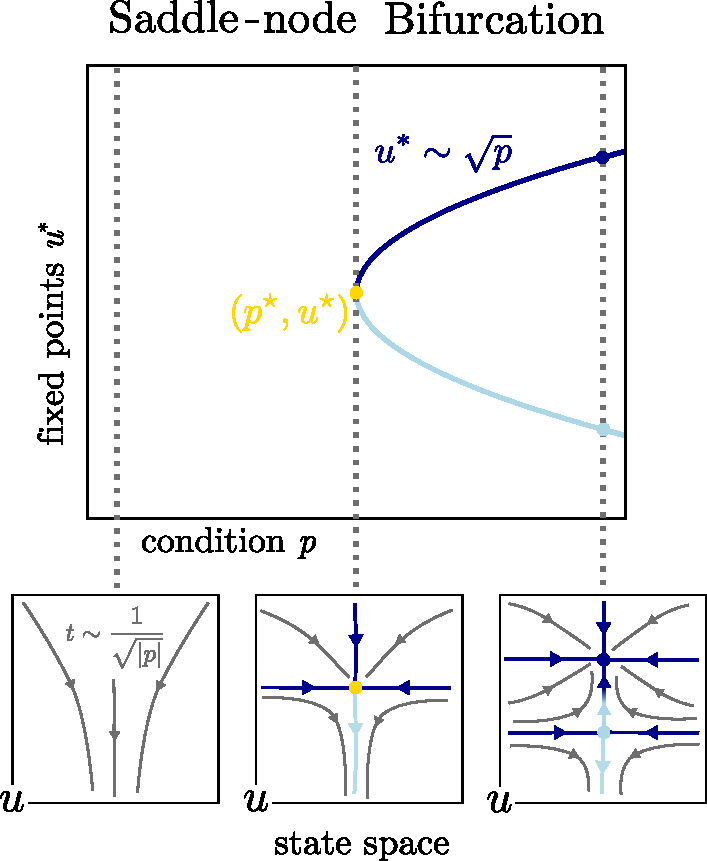
\includegraphics[scale=0.7]{saddle-node} 
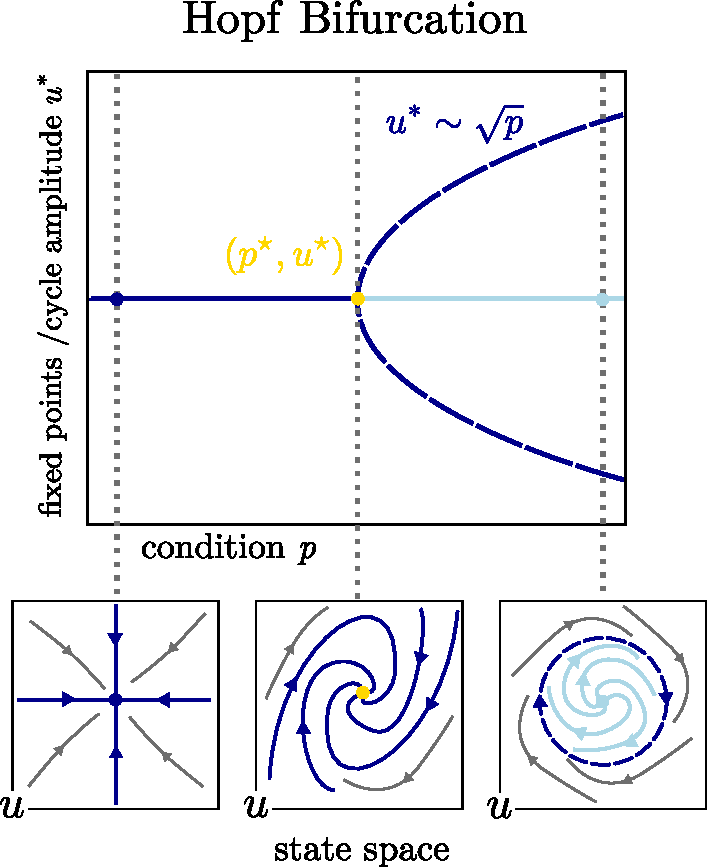
\includegraphics[scale=0.7]{hopf}
\caption{All bifurcations}
\label{fig:bifurcations}
\end{Figure}

\subsubsection{Dynamic Bifurcations}
Another category of bifurcations involves limit cycles, which emerge from fixed
points where the linearised Jacobian eigenvalues have no real part. Limit cycles
have circulating field flow as shown in Figure \ref{fig:stability} along the
$\mathrm{Tr}[\mathbf{J}]=0$, $|\mathbf{J}|>0$ axis.

Note how oscillations emerge at small amplitudes in the Hopf bifurcation,
whereas the large amplitude oscillations may instantly emerge in an infinite-period
or cyclic-fold bifurcation. In Figure \ref{fig:limitcycles} the shaded regions
represent the peaks and troughs of the oscillations.
\begin{Figure}
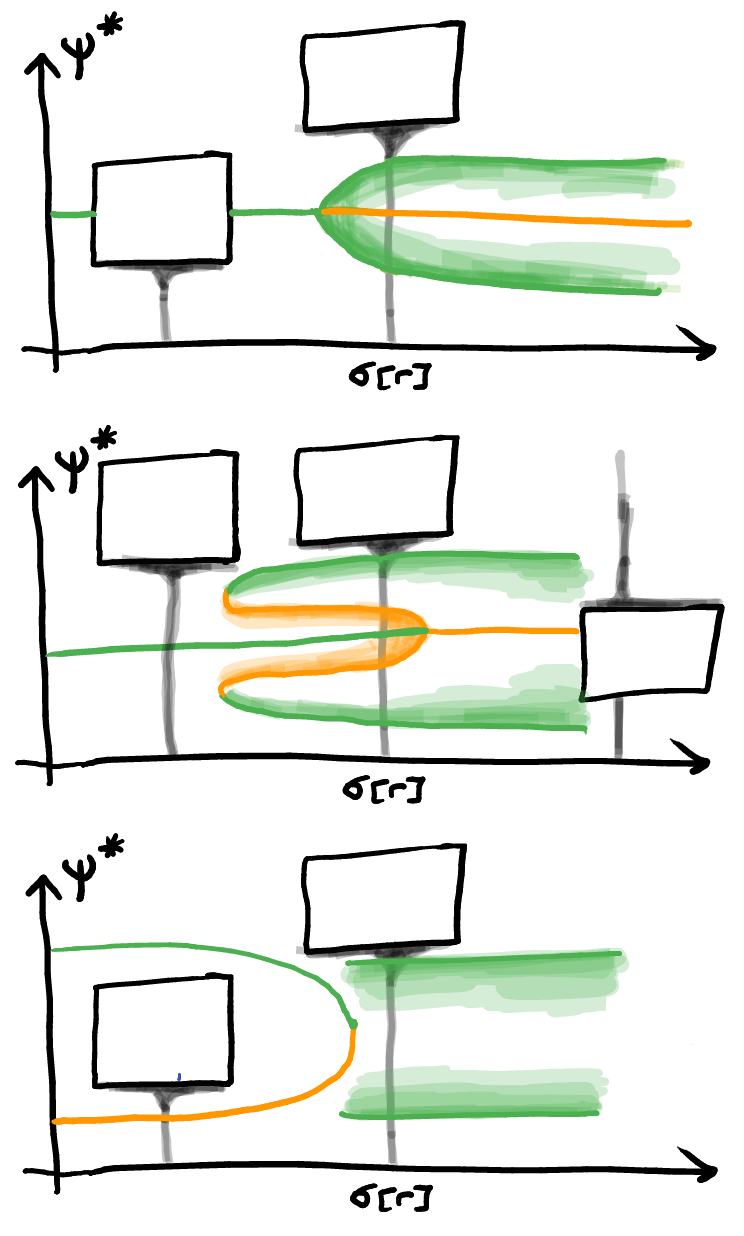
\includegraphics[scale=0.35]{figures/limitcycles}
\caption{Hopf, Cyclic-fold and Infinite-Period bifurcation diagram showing
\textcolor{Green}{stable} and \textcolor{orange}{unstable}\\ fixed points
and limit cycles as a function of parameter $\sigma[r]$.
Insets show nullclines [tbc]}
\label{fig:limitcycles}
\end{Figure}

\subsubsection{Parameter Continuation}

\subsection{Spatially Extended Systems}

If $\rates$ contains spatial derivatives, additional conditions on $u$ with respect to spatial variables $x\in\Reals^D$, where $D$ is the dimension of the space considered, must be supplied to give a unique solution $u(x,t)$.



\subsubsection{Turing Bifurcations}
When studying spatio-temporal dynamics of organisms, a popular choice is to incorporate a diffusive term that models the exchange of matter between spatial locations
\begin{align}
	\partial_t
	\psi &=
	\mathbf{\Gamma}\omega(\psi|\mathbf{\Gamma})
	\label{eq:reaction}
\end{align}


A bifurcation diagram tracks changes in attractors such as fixed points $\steady$ and limit cycles $\cycle(t)$ in response to changes in control conditions $p$.  In the next section we will see how fixed points and limit cycles are characterised with linear stability analysis

this can be done using 
In this thesis we extensively use the library \texttt{DifferentialEquations.jl} \cite{Rackauckas2017Differentialequations.jlJulia} for numerically solving differential equations and \texttt{BifurcationKit.jl} \cite{Veltz2020BifurcationKit.jl} for calculating bifurcation diagrams. 

Partial observation can be modelled explicitly with latent variables \cite{} or the explicit modelling of system and measurement device as is done in control theory \cite{}. For the scope of this thesis we will let the modeller have complete freedom on how to choose relevant state variables $u\in\Reals^N$ and write down their own set of differential equations, with unknown parameters $\theta\in\Reals^M$ of the form

\section{Applications in Cell Biology}
\label{section:applications-cell-biology}

\subsection{Genetic Switches \& Phenotype Boundaries}
These equations can originate from mean-field approximations of the chemical master equation \cite{} representing biochemical reaction networks \cite{}. This typically yields models with a large number of parameters $M$ and states $N$. The equations could have also undergone a series of quasi-steady state approximations \cite{} yielding hill-functions. Various other model reduction methods exist \cite{} in an attempt to reduce the number of state variables $N$ and parameters $M$.

\subsection{Populations of Neurons}

\subsubsection{Neural Differential Equations \& Gaussian Processes}
While principled derivation from microscopic rules exist, often the the number of variables $N$ participating in the mechanism under study becomes intractable. When the desire for predictive performance out-weighs the desire for mechanistic explanations, the states $u$ are chosen to be the observable subset for which we have data, and the right-hand side $\rates$ can be a machine learning model such as a neural network or Gaussian process \cite{}. In this case the number of parameters becomes much larger than the number of states $M\gg N$. A recent breakthrough in back-propagation through differential equation solvers \cite{} has made these models tractable in optimisation routines, and popularised them in literature \cite{}.


\subsubsection{Stochastic Differential Equations}


\subsection{Self-organised Patterns \& Development}

In this section we would explore the geometrisation of phase space, lyapunov
exponents and universality. Perhaps a discussion on phase transitions and
the relation to Landau-Ginzberg approaches is required.
Maybe also periodic orbit theory? Depends how useful it is.
\subsubsection{Reaction-Diffusion}
Here we first introduce diffusion macroscopically by simply adding the laplacian
to mean field equation $\eqref{eq:reaction}$. We introduce the turning bifurcation and
show how linear stability analysis is insufficient to capture pattern formation
and rich inhomogeneous steady states. A promising approach may be geometrisation
of the moving local equilibria \cite{Halatek2018}.

\section{Phenotype Inference with Machine Learning}
\label{section:phenotype-inference}
\begin{itemize}
    \item Preface on SciML community and gray-box modelling
\end{itemize}

\subsection{Classification and Regression}
\begin{itemize}
    \item Logistic regression
    \item Nearest neighbour methods
    \item Mixture Models
\end{itemize}

\subsection{Dimensionality Reduction Methods}
\begin{itemize}
    \item UMAP and Tsne
    \item Sloppy parameters and identify-ability
\end{itemize}

\subsection{Clustering Methods}

\section{Applications in Flow Cytometry}
\label{section:applications-flow-cytometry}


\subsection{Immunophenotyping Panels}


\subsection{Inferring Bifurcations from Data}

In sections \ref{inference:abstract} -- \ref{inference:impact} we assume that the bifurcation data $\targets$ with respect to the experimental control condition $p\in\Reals$ is known or already extracted from raw data. We can break down the extraction process into steps: steady state inference, field inference and fixed-point inference; each discussed separately in its own subsection. These steps are sequenced together into two possible routes towards bifurcation data $\targets$ as depicted in Figure \ref{fig:inferring-bifurcations}.

At best we could have state trajectory data like single cell trajectories extracted via segmentation and tracking in fluorescence microscopy movies (for example the data acquired using the CellASIC platform in Figure \ref{fig:double-exclusive:bistability}c). Having the the state as a function of time $u(t)$, sampled at sufficiently broad initial conditions $u(0)$, enables the \emph{non-parametric} estimation of field geometry $F(u)$. We can then extract important state-space structures, such as stable and unstable fixed points, their eigenvalues $\lambda$, from the field geometry $F(u)$ at different values of the control condition $p$, and hence identify possible bifurcations.

\begin{Figure}
    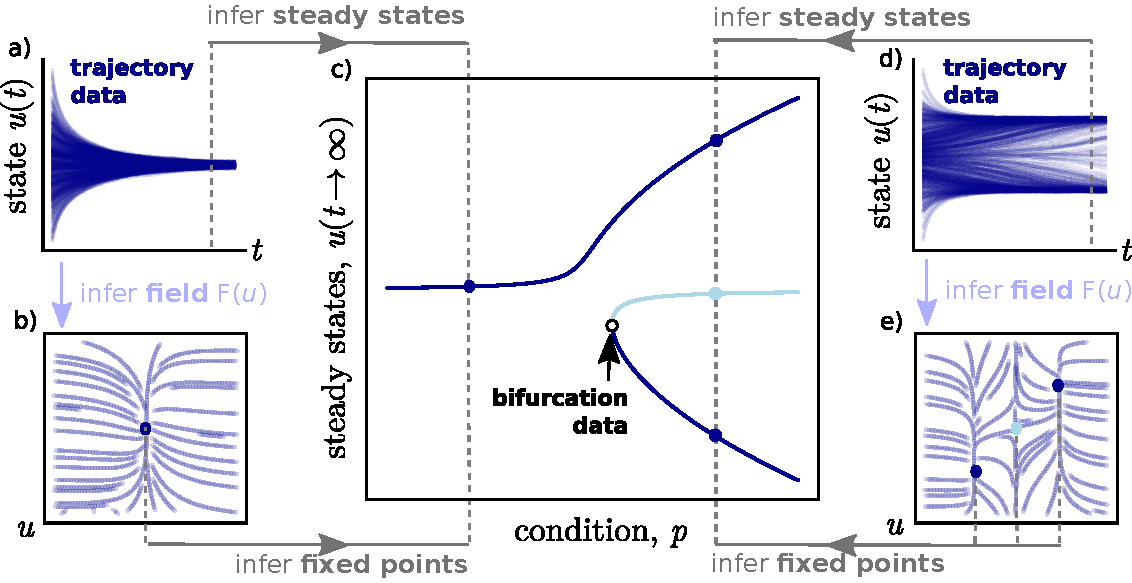
\includegraphics[width=14cm]{inferring-bifurcations}
    \caption{Bifurcation point extraction along the condition $p$ via two possible routes: steady state inference (a,d$\rightarrow$c) and fixed point inference (a,d$\rightarrow$b,e$\rightarrow$c). The fixed point inference route requires the geometry of the field $F(u)$ at different values of the condition $p$ and yields additional information about unstable fixed points.}
    \label{fig:inferring-bifurcations}
\end{Figure}
Data on steady states $u(t\rightarrow\infty)$ are more abundant and typically found in flow cytometry measurements. It is possible to infer the steady state manifold directly from such data (Figure \ref{fig:inferring-bifurcations} a,d$\rightarrow$c) but we would not be able to extract information on unstable fixed points or eigenvalues $\lambda$ of state-space structures. Since the criteria for bifurcations are not directly accessible, indirect measures (such as the population separation that can be seen in Figure \ref{fig:double-exclusive:flow-hysteresis}) must be used to extract bifurcations.

\subsubsection{Bifurcations via Steady State Inference}
\label{section:steady-state-inference}

Suppose we would like to detect a cusp bifurcation and limit points in a cell population with respect to two experimental control conditions $p,p\prime\in\Reals$. We can set up a serial dilution along the columns for $p$ and along the rows for $p\prime$ in two 96-well plates. Cells allowed to grow in exponential phase in a finite concentration of either $p\ll p\prime$ or $p\gg p\prime$. Let us call this the \emph{priming} stage of the protocol as shown in Figure \ref{fig:cusp-sampling}a, resulting in two cell populations: $p$-primed cells and $p\prime$-primed cells. The priming concentrations must be chosen sufficiently high so that the resultant population states lie either side of the cusp. The two populations are transferred into separate 96-well plates containing the dilutions of $p,p'$; we call this the \emph{conditioning} stage in Figure \ref{fig:cusp-sampling}a.

\begin{Figure}
    \includegraphics[width=14cm]{hysteresis}
    \caption{Protocols (a) for extracting limit points with respect to conditions $p,p'$. Steady state distributions (b). Similarity measure (c)}
    \label{fig:cusp-sampling}
\end{Figure}

The cells are then transferred into a flow cytometer, gated for live singlets and processed with relevant compensation and auto-fluorescent normalisation, which would produce the population distributions $P(u)$ for the $p$-primed cells and $Q(u)$ for $p'$-primed cells in each well. By overlaying distributions $P(u),Q(u)$ for each well, a figure similar to Figure \ref{fig:cusp-sampling}b (or Figure \ref{fig:double-exclusive:flow-hysteresis}) can be produced. Finally, the limit points can be defined by a level set of distribution similarity measure $D(P||Q)$ in the $p,p\prime$-plane as shown in Figure \ref{fig:cusp-sampling}c. This similarity measure could be Kullback–Leibler divergence or something as simple as the distance between distribution medians. The level set must be some small positive amount $\epsilon$ above zero, picking out the onset of dissimilarity between steady state distributions $P(u)$ and $Q(u)$, and hence the onset hysteresis. We can define the limit points as
\begin{align}
    \targets = \{  (p,p\prime) : D(P||Q)=\epsilon, \epsilon>0 \} 
\end{align}

This approach may break down if multi-modal distributions exist in the data. This would be the case if something happened to prevent a subpopulation of cells to switch from one state another other. Reasons for this could include too much cell burdon or not enough time given for cells to reach a steady state. In this case, quantifying the efficiency of switching from either side of the cusp could be a quantity of interest.

This approach would not work for extracting dynamic bifurcations such as \emph{Hopf} since only steady state information is available. Furthermore, the accuracy of this method is subject to noise amplitude. This method works well for cases where changes in the number of stable steady states can be resolved in the measured steady state distributions.

\begin{itemize}
    \item \todo[inline]{quantify efficiency of switching?}
\end{itemize}


\subsubsection{Non-parameteric Vector Field Inference}
% Non-parametric ___ using Gaussian Process regression
\label{section:field-inference}

In this early days of this thesis, we investigated whether it was possible to transform the time-domain data into state-space. This approach, and related works, are discussed in this section and can in principle be used with the microfluidic fluorescence microscopy data for parameter inference.

Consider we are given $K$ cell trajectories $\mathcal{D}_1$, $\mathcal{D}_2$ ... $\mathcal{D}_K$, each containing $N$ noisy observations of the state of the cell. Let the cell state be represented by state vector $u(t)\in\Reals^N$ which is hypothesized to obey a set of ordinary differential equations of the form \eqref{eq:differential-equations}. Instead of integrating the equations \eqref{eq:differential-equations} we would find an estimate for the derivative of the trajectories $\hat{f}$.

This is known as the \textit{smoothing} step \cite{Gugushvili2012Smoothing} should be done using unsupervised methods, for example with Gaussian Process Regressors \cite{Seeger2004GaussianLearning.} as shown in in Figure \ref{fig:inferred-cycles}. This requires the inversion of an $K'\times K'$ data matrix where $K':=\sum_k |\mathcal{D}_k|$ is the total number of trajectory data points. This has a computational complexity $K'^3$ which is only tractable with sparse datasets.

Let the region $\partial\mathcal{D}$ be a boundary defined by the Delaunay tessellation of the input data. Let us define the estimate $\hat f$ only within the region $\partial\mathcal{D}$ so that there are no extrapolation artefacts. For the Gaussian Process approach the estimate would be
\begin{equation}
    \hat{f}(u)\sim
        \mathcal{N}(\,\mu(u) ,\Matrix{\Sigma}(u)\,)
    \quad\mathrm{for}\quad u\in\partial\mathcal{D}
\end{equation}
\noindent where at any given state $u$ the field estimate $\hat{f}$ is generated by Gaussian distributions of mean vector $\mu$ and covariance matrix $\Matrix{\Sigma}$.Solving for these requires a choice of matrix-valued kernel function $\Matrix{K}(u,v)$ which encodes our knowledge about the local structure of the field. Sophisticated kernels for learning vector fields exist \cite{Fuselier2017ADecompositions} for decomposing fields in conservative and solenoidal components, which aid in localising fixed points and cycles.

The simplest choice of kernel assumes the components are independent and have a finite correlation length $\gamma$, such as Gaussian radial basis functions. Here $\Matrix{I}$ is the identity matrix and the hyperparameter $\gamma$ has to be optimised.
\begin{equation}
    \Matrix{K}(\Vector{u},\Vector{v}) = \Matrix{I}\,\mathbb{e}^{-\gamma|\Vector{u}-\Vector{v}|^2}
\end{equation}

The second step is called \textit{matching} where the estimated field $\hat{f}$ is used as an optimisation target against some parametrised function $\rates$ with unknown parameters $\theta$.

In our setting we would like to match the geometry of the field but not its magnitude; in this sense we are focusing on the qualitative aspects of the dynamics of a set of differential equations, rather than the quantitative dynamics or kinetics. This could be achieved with the following objective function
\begin{equation}
    \mathcal{L}(\theta|\mathcal{D}) := \e^{-\frac{\hat{f}\cdot\rates}
    {|\hat{f}||\rates|}}
\end{equation}
\noindent where the cost is minimal when the data derivative $\hat{f}$ and the parametrised model $\rates$ point in the same direction and maximal when they point in opposing directions.

\begin{Figure}
    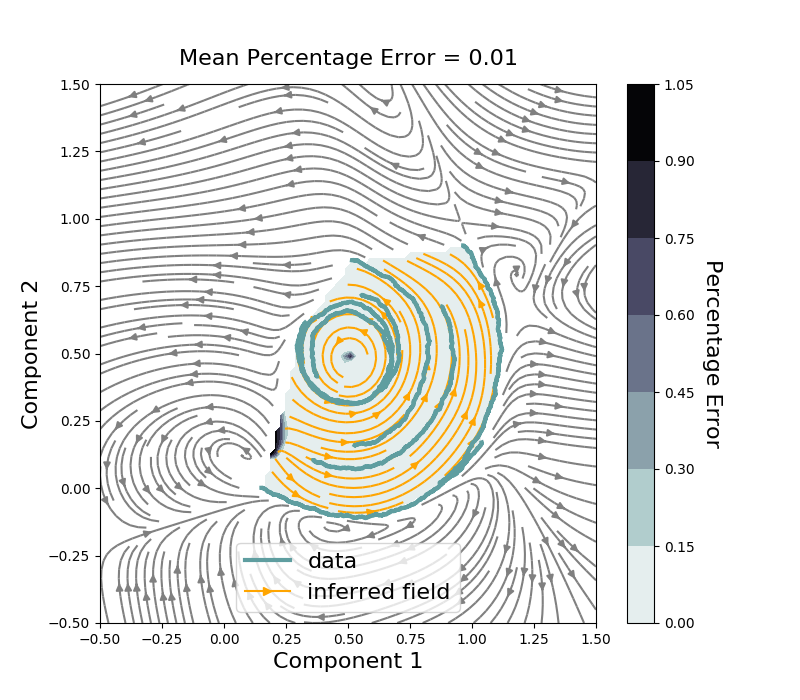
\includegraphics[width=125mm]{figures/cycle-2.png}
    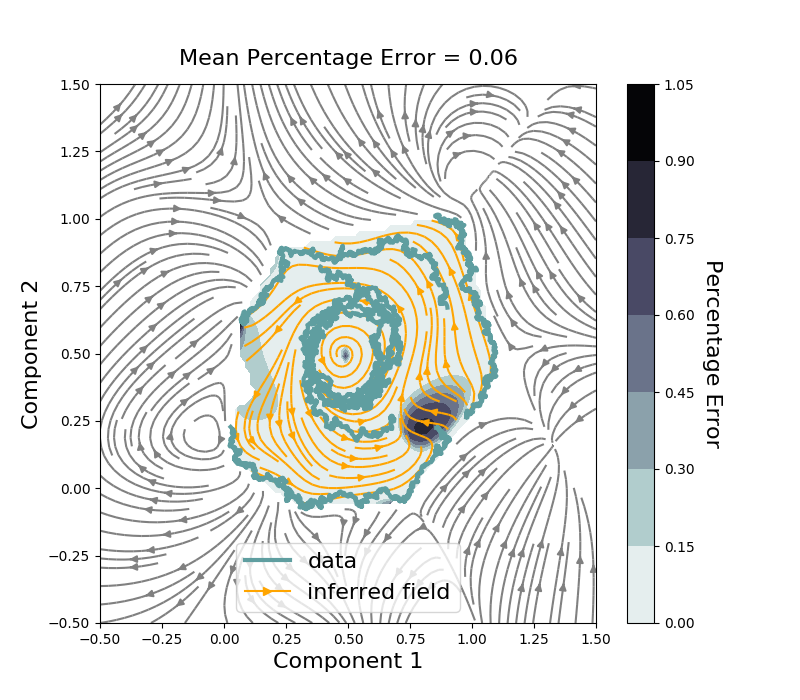
\includegraphics[width=125mm]{figures/cycle-1.png}
    \caption{Gaussian process regressors estimating derivative of the trajectories $\hat{f}$ from example trajectory datasets $\mathcal{D}_1$ ... $\mathcal{D}_K$ with varying signal to noise ratios. Interpolation error $E$ is shown as a heatmap; extrapolation fails}
    \label{fig:inferred-cycles}
\end{Figure}

Although we are getting close to focusing on qualitative features of a model, this objective function is still sensitive to the locations and shapes of fixed point and limit cycles. What if we cared about even higher-level features such as the number of fixed points? Or perhaps whether a system oscillates or not? This is where the language of bifurcation theory described in Chapter \ref{chapter:background} is optimally suited for this task, but fist we need to discuss how to set up experiments to detect bifurcations from flow cytometry data.

\begin{itemize}
    \item \todo[inline]{Vector field estimates too noisy to get bifurcation points?}
    \item \todo[inline]{Divergence and the stability of fixed points}
    \item \todo[inline]{Curl and limit cycles. How does this relate to hopf example \ref{fig:inferred-cycles}}
    \item \todo[inline]{Do we need a bistable example?}
\end{itemize}

The accuracy of the cell trajectories is limited by cell segmentation and tracking algorithms. Initial investigations into this approach also suggested that trajectories need to be of sufficient temporal resolution and sampled from a wide variety of initial conditions. Such data is not widely available and ultimately we decided to focus on a method that could be used with a well-known workhorse in biomedical research: flow cytometry.

\subsubsection{Fixed Point Inference}
\label{section:fixed-point-inference}

\subsection{Multiomics Integration}